\chapter{State of the Art} \label{chap:State of the Art}
Summary of this chapter will come here ... 

\section{Reactive Systems}
The state is essential and important part of Reactive systems because the state of the system gets changed as result of processing of events. According to the Reactive manifesto \citep{reactiveManifesto}, Reactive systems responds in a timely manner even in the case of failure or variable workload and ensure loose coupling between its components by using asynchronous message passing.
Reactive systems are the systems that can react to events (Event-driven), that should react to load (Scalable), that should react to failure (Resilient) and that should react to its users (Responsive). we can think web application as a reactive system, where Events happen on DOM \citep{W3DOM} elements, results in a change in state which can be visible or hidden to end user. \citep{Zanarini:2014:MRS:2637113.2637120}.

\section{Afore Reactive Programming}
Before the invention of high-level programming languages like C or Pascal, programmers had to write computer programs in machine or assembly language. In the era of 1980's object-oriented concepts made high-level programming languages more modularized. An American professor of computer science expressed his dream about the future of programming languages in his article. He dreamed at that time that as high-level programming language escape programmers from the complexity of machine language, higher level programming systems can provide means to understand and manipulate complex systems and components. I think with today's functional and reactive programming paradigms, his dreams comes partly true \citep{Winograd:1979:BPL:359131.359133}.
This section will present some programming paradigms used in past to implement reactive systems. Next sections will have more focus on reactive languages and libraries.

\subsection{Observer Pattern}
This pattern is being used for ages to implement interactive applications. This pattern does not eliminate the problems of the manual approach of propagation of change. But it does modularize the process of propagation of any change to its dependents. Observer pattern defines dependency between objects so that if one object changes state, all of other dependent objects are notified automatically \citep{Gamma:1995:DPE:186897}. With observer design pattern amount of code for handling events, is quite large which leads to complex and error prone code. This report Deprecating the Observer Pattern \citep{EPFL-REPORT-176887}, proposed a way to minimize the amount of code in an application to handle events by abstracting the logic of event handling as part of programming language.

\subsection{Iterator Vs Observer Pattern}
Iterator pattern allows consumer to pull data from any data structure progressively, one item at a time. While observer pattern do almost same thing but in this case producer sending / pushing data to the consumer when data is ready. Consumer gives callback to data producer and then producer calls the callback to push data to consumer. In iterator pattern, the consumer decides when to pull data from producer and in observer pattern, its producer decide when consumer going to receive data. Both patterns are explained in detail in book 'Design Patterns: Elements of Reusable Object-Oriented Software by Gang of four' \citep{Gamma:1995:DPE:186897}. Observer pattern is pretty well suited for UI events, and iterator pattern is for traversing different type of collections in a consistent way.

\subsection{Callbacks}
Before Reactive programming paradigm, Events handling in Interactive applications were done with the help of asynchronous callbacks also know as event handlers. 
Instead of blocking program execution while waiting for the result of any asynchronous computation, Callbacks are used to receive the results of asynchronous task by registering a method that does execute, when result of computation is ready. Nesting callbacks to handle multiple asynchronous tasks in a program mostly leads to a well known problem called 'callback hell' \citep{Kambona:2013:ERP:2489798.2489802} also termed as asynchronous spaghetti \citep{SMLI-TR-2007-166}. Callback hell basically is a state of the program that tries to benefit from callbacks but on the other hand, it gets so complex to understand, maintain and give the reason about that code. Another drawback of using callbacks is that it needs to shared mutable state and Event listeners have a hard time of being composed.

\subsection{Promises}
In JavaScript, term promise is used for a proxy object that represents a future value that is not available initially and yet to be computed in future \citep{Kambona:2013:ERP:2489798.2489802}.  In other programming languages, promise may be called as future, delay or deferred. Promises are already implemented by some open source libraries with minor difference in syntax include Q, jquery, deferred.js, vow. In JavaScript, promises becomes standard with the release of ECMAScript version ES6 in 2015 \citep{ecmaScriptPromise}.
Replacing nested callbacks with promises gives more structure to code, that becomes easy to handle and understand. Because promises are first class objects that's why they are also easily composable \citep{Kambona:2013:ERP:2489798.2489802}.

\subsection{Imperative vs Functional programming}
Imperative programming paradigm prescribes the computer, what to do and step by step procedures are used. It is closer to machine language. In imperative programming, we commonly use if-structure, loops, functions etc. C, Java are the examples of imperative programming languages. Imperative programming is easy to understand, debug. Normally it has objects and state variables define but the code can be lengthy and hard to scale.
In imperative programming, there is freedom of changing values anytime but consequences of those changes have to deal manually \citep{Edwards:2009:CR:1639950.1640058}.

In functional programming paradigm, we describe the end results, and we use function calls, higher order functions, recursion etc.. Pure functional approach has no memory / IO side effects. Very less code which is easy to scale. A functional programming paradigm is not well suited for simple tasks. The code in functional approach is a bit complex to understand. In functional programming, the task is achieved by calling a function without knowing the details of how operations are performed. Scala, Haskel, Lisp are based on functional programming paradigm.

\section{Reactive Programming}
In recent past years, software applications have been changed dramatically and becomes more and more interactive. Applications needs to be more responsive to the events happening outside and within an application environment. If system is responsive than users of that system tends to stays with it, and non responsive systems lose its users pretty quickly. Another important property of modern days applications is scalability, that means system should be able to respond in case of load. To fulfil above mentioned requirements sequential programming techniques are not enough because of unpredictable behavior of events and their effects. Before this programming model, any change in state, its effect and order of performed actions was managed by programmers manually, that was very complex and likely to fail or make errors in results \citep{Edwards:2009:CR:1639950.1640058}.
Reactive programming came into existence as a programming model that assist event driven and interactive application development. It provides abstractions, to represents values that change over time, to manage events handling, to manage state changes and to manage dependencies among each other. The reactive programming model is similar to spreadsheet model in the sense of handling computation dependencies automatically, as in the spreadsheet changing the value of one cell can effect on other cells automatically \citep{Bainomugisha:2013:SRP:2501654.2501666}. In Reactive programming if some variable is defined as time changing value, then it means every time there will be a change in the value of that variable, reactive language or library will automatically propagate that change to all part of the program that depends on this particular variable.
For example, if we have expression var a = b + c; Traditional programming languages will treat this expression as just an assignment of the sum of values of b and c, while in RP this is treated as a constraint. So whenever the value of b or c gets change than the value of a will be updated automatically.
This programming model has more emphasis on scalability and responsiveness, so we can say that Reactive programming is a programming model that help us to build a scalable architecture that is resilient and quick to react to any change. Event-driven programming model has more focus on handling single events and reactive programming focuses on data flows and propagates the change all over.
So far most of the reactive languages were implemented on top of functional programming paradigm, that's why also known as functional reactive programming. 
Fran, Haskel , Frame, Flapjax, Scala React, Reactive X, Bacon etc ..

\subsection{Reactive Programming With Javascript}
JavaScript is the most famous programming language for developing client-side web applications and overall was ranked as the seventh most popular
programming language in February 2017 \citep{TiobeIndex}. JavaScript is considered as a dynamic programming language because it provides features at runtime that non-dynamic programming languages provide during compile time. Treating functions as objects and allowing insertion and evaluation of code at runtime using 'eval', makes JavaScript more dynamic \citep{White2010}. Dynamic nature of JavaScript also attracts web application developers to write server-side script also in JavaScript, which becomes possible, more recently, with node.js \citep{NodeJs}. Several mobile platforms including IOS, Android, Windows, Blackberry and Firefox OS, support applications developed in JavaScript. The best thing about JavaScript is that applications developed using JavaScript are portable. Most of the modern day devices have browser to run JavaScript applications \citep{Richards:2010:ADB:1809028.1806598}.
Web applications nowadays are no more static HTML pages, they become more interactive and complex, contain asynchronous behaviour \citep{6068340}. Before reactive programming, above mentioned requirements were managed with the help of callbacks, promise pattern but those all are difficult to handle and mostly are error prone. To manage this advancement there are some libraries have been developed in recent years to implement reactive programming paradigms as an extension to most commonly used client side in the web world that is known as javascript. Although nowadays javascript is also being used to develop server side code in the form of node.js. We will discuss two most famous libraries in detail as these two will be the main focus of this thesis.

\subsection{ReactiveX and RxJS}
ReactiveX is basically a pool of libraries based on different well-known programming platforms like Java, PHP, JS etc.. It provides libraries on top of these different programming platforms, to add abstraction to those languages, to able to program in more declarative and reactive manner. Sometimes the term Functional reactive programming has been misused for ReactiveX library but Functional reactive programming is bit different. The major difference between these two is that functional reactive programming operates on values that change continuously over time, while ReactiveX operates on discrete values that are emitted over time \citep{reactivex}. 
The Reactive extension for JavaScript, RxJS is set of libraries to develop asynchronous and event-based programs. Basically, RxJS compose of three components named as Observable, Operators, Schedulers. Observable are used represent asynchronous data streams. Operators are used to transforming those event streams from one form to another and use schedulers to handle concurrency in these event streams \citep{rxjs}.

\subsection{Important Concepts of RxJS}
\subsubsection{RxJS Reactive Pattern}
In ReactiveX observer subscribe to an observable and react to items emitted by an observable. This concept ensures the concurrency because observer does not need to block itself while waiting for data from an observable. Marble diagram is a great way to visualize this pattern. In following figure marble diagram is used to explain observable and transformation of observables to another form.

\begin{figure}[!h]
	\centering
	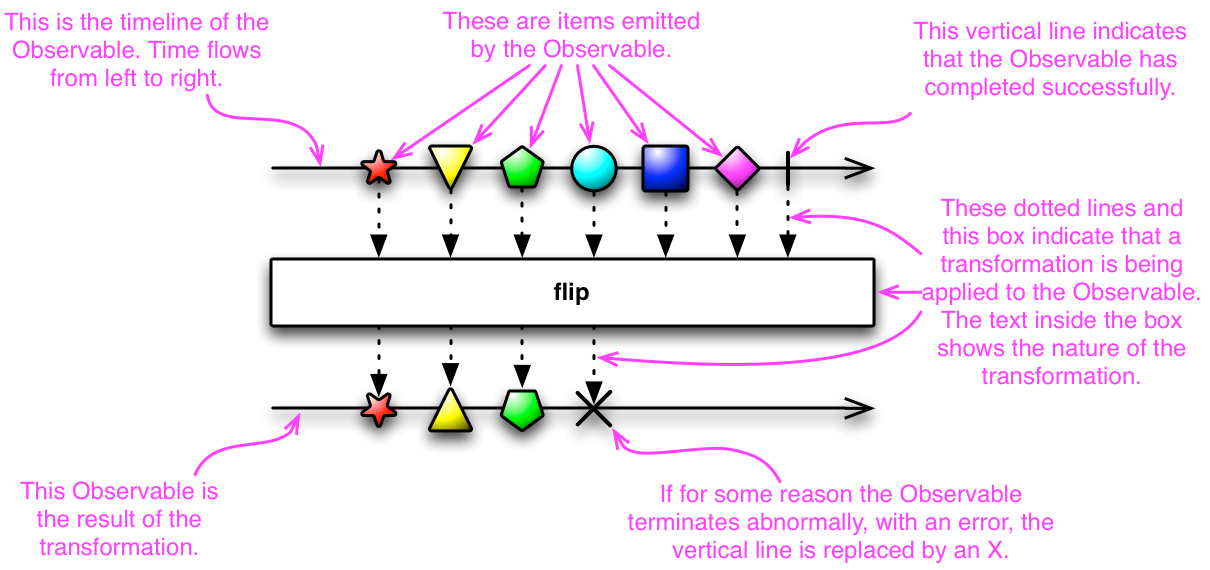
\includegraphics[scale=0.5,trim=0 0 0 0]{gfx/rxjs-reactive-pattern2.png}
	\caption{Reactive pattern}
\end{figure}

\subsubsection{Observable and Observer}
Observable is the basic building block of RxJS. It is the name of another abstract data type just like an array and other collections in programming languages. It represents any set of values over any amount of time. Observable contains a sequence of values that a data producer pushes to the consumer. Observable also can signal to its listener that its has been completed and will not send data anymore. With an array, all data is stored in memory and with Observable, there is no data stored in memory and items arrive asynchronously over time. We can also name observable object as a provider because observable object represents the object that sends notifications to the observer object.
Observable gives us object that represent event stream and we can use that object to perform different methods on that object similarly as we do with array like we can traverse an observable as we traverse an array. In RxJs Observable can be of two types , Hot or Cold. Hot observable starts emitting values as soon as it has been created and cold observable starts emitting data when an observer subscribe to it.

\subsubsection{Operators}
Operators give real power to ReactiveX. RxJS provide a bundle of operators that we can perform on Observables to transform and event stream to another with different properties. List of those operators with details is available in the reactiveX online documentation \citep{reactivexOperators}.
Most of those operators operate on Observable and produce another observable that allow chaining operators one after another.

\subsubsection{RxJS Example}
Example code with explaination here ..

\subsection{Bacon.js}
Bacon.js is functional reactive programming library for javascript that assists to deal with asynchronous nature of javascript code. It is comparable to Underscore.js \citep{Underscorejs}, that is a javascript library that provides a collection of useful functional programming helpers (utilities) for common tasks/use cases, like map, filter, invoke etc..
Underscore.js is for data which is available already like arrays. Bacon.js turn the way of handling individual events with imperative programming model into functional programming model and works on events streams. So using this library will reduce the complexity of handling events individually into code that will look more logical, easy to understand and functional.

\subsubsection{EventStream and Property}
In Bacon, these are two flavors of Observables. EventStreams and Property are two basic concepts of Bacon.js that are basically known as events and behaviors in the literature of FRP.
EventStreams are sources of events. For example mouse clicks, keyboard events can be model into an EventStream object. EventStreams are composable means we can combine several EventStreams objects to create resultant EventStream.
Property that is also known as behaviors and signals is an abstraction for the values that vary over time \citep{GithubFRP}.
Properties are very similar to EventStreams and share most of the functionality with EventStream but Property have also concept of current value and we can create a Property from event stream by using toProperty or scan method \citep{BaconProperty}.

\subsubsection{Bacon Example}
Example code with explaination here ..

\section{Debugging and Tools Support}
In software engineering literature, the process of finding errors in a computer program is called debugging. The error can be logical or syntax error. Debugging tools are always helping hands of programmers whether they are trying to find an error in their own program or they are trying to understand the working of programs written by other developers. Mostly debugging tools gives its users some visual representation of the code and gives user privilege to control, on how the program executes. 

\subsection{Debugging JavaScript}
Dynamic and reflective nature JavaScript makes it hard to debug and analyse JavaScript code \citep{Richards:2010:ADB:1809028.1806598, Schafer:2012:RTD:2328876.2328885}. Before the advancement of browsers, application developers mostly rely on 'alert' statement to inspect values of variables and the output of functions but for this, they are required to change the code. Besides using console.log and debugger statements, now modern browsers gives more built-in debugging functionalities, that developers can use to debug JavaScript program. Programmers can set breakpoints to halt the execution of a program and can examine the complete context in which any statement or function executes. Developers can also observe performance and memory consumption of code. There is a long list of similar features but these are out of the scope of this work.
If we compare debugging support from language itself, then we will get to know that JavaScript language provides very limited support for debugging. It does not offer any API to for debugging purpose. Unlike JavaScript other programming languages like C/Java provides Apis or packages to developers that can be used for debugging purpose. For example in Sun Java Development Kit (the JDK) includes the Java package sun.tools.debug, which provides a simple interface into the Java Virtual Machine. This API allows another program, probably a debugger, to connect and communicate with the Java Virtual Machine to get low-level information about a currently executing Java application \citep{vanderburg1996tricks}. Another reason why it is hard to debug JavaScript code is that JS code does not need to compile before execution, as other languages, so all bugs can only be found at runtime.

\subsection{Jalangi}
\begin{figure}[!h]
	\centering
	\includegraphics[scale=0.5,trim=0 0 0 0]{gfx/HowJalangiWorks.png}
	\caption{How Jalangi Works}
\end{figure}

Jalangi is dynamic analysis framework for JavaScript applications. Using this framework, it becomes possible to monitor every operation of the JavaScript application and its API make it possible to write own program analysis modules. Jalangi framework works independently of the platform where the code eventually runs. Basically this framework instrument all JavaScript code given to it and create hooks in resultant code. Hooks inserted by this framework are used to monitor each operation at runtime, like read from, write to variable, function calls etc.. \citep{Sen:2013:JSR:2491411.2491447}

Above figures explain about the working of Jalangi framework, First of all, Jalangi instrumentation module takes JavaScript code and instrument that code to be execute in the browser. Beside this instrumented code Jalangi runtime code also executes in browse, that is the Jalangi runtime framework code which implements those hooks called in instrumented code. Those hooks keep the semantics of the target code and invoke callback functions defined in User written analysis code. The user-written analysis is the code written by third-party program analysis developers, overriding those predefined APIs allows to intercept those execution events and do program analysis.

\begin{lstlisting}[language=JavaScript, caption=Jalangi Instrumentation]
// Before Instrumentation
	x = y + 1
// After Instrumentation
	x = Write( 'x' , Binary ( '+' ,  Read( 'y' , y ) ,	Literal(1) , x )
\end{lstlisting}

The first code snippet is before instrumentations and the second one is the code after instrumentation is done by Jalangi. Jalangi framework runtime code implements those hook callbacks (Read, Write, Binary, Literal etc .
This framework can be used to check different kinds of correctness bugs and performance bugs, doing various program analysis (e.g., debugging, Performance analysis, Monitoring dynamic behaviors, Record and replay, runtime call graph etc..
We use this framework as in our extension to find the reference of a node of dependency graph to JavaScript variable name. Details of this usage will be presented in further sections.


\subsection{Debugging in Reactive Programming}
Nowadays advanced debugging tools are an essential part of good IDE, but those are not sufficient to handle the immense difference in approaches of imperative and reactive programming \citep{Salvaneschi:2016:DRP:2884781.2884815}.
So for reactive programming, debugging tools intends to manage conceptual change of reactive programming as compared to traditional imperative programming. As Reactive programming paradigm is still new and emerging model that's why we don't have many examples of tools that are build to debug reactive programs. 
In RP Debugging technique model reactive application into dependency graph where nodes represent the values/signal that may change over time and edges between them depicts dependency among various signals. They have also implemented RP Debugging technique as Eclipse plugin to debug software in reactive style \citep{Salvaneschi:2016:DRP:2884781.2884815}. This thesis is result of inspiration of above-mentioned technique. 

\subsection{Debugging Reactive Extensions of JS}
Bacon and RxJS are already introduced in above sections xx will be the main focus of this thesis. Debugging asynchronous code is not an easy task. As mentioned before that RxJs and Bacon work with streams of events asynchronously. That's why it's not feasible to use traditional browser developer tools to debug RxJS and Bacon based applications.
Like other reactive programming languages or extensions, there is no debugging tool available for these libraries. These libraries are getting fame day by day but still missing tools support that can help developers to debug and understand programs written in these libraries.
In this article \citep{StaltzAticleHowToDebugRxJS}, the author explains why traditional dev tools are not enough to debug RxJS code. Because applications developed using these libraries are abstract code and not procedural code anymore, that is why browser developer tools and breakpoints do not help while debugging or understanding code. In this article, the author wrote that to debug the RxJS application you have to rely on drawing dependency graph and marble diagrams by hand. The dependency graph is introduced already, Marble diagram is the visual representation of input and output of operators available in these libraries \citep{StaltzMarbleDiagrams}.
So it is badly required to extend existing debugging tools to support debugging for JS libraries build to implement the concepts of reactive programming.
This thesis is the first step towards having debugging tool for these libraries. We implemented an extension to chrome dev tools where developers can visualize and debug code written in RxJS or Bacon library. Details of this tool will come in coming chapters.

\section{Related Work}

\subsection{Omniscient Debuggers}
Log-based debugging and breakpoint-based debugging are two traditional debugging techniques. First one requires manual modification of source code to trace program execution whereas the second one allows setting breakpoints within source code to step into code execution. Omniscient debuggers overcome the issues of traditional debuggers and combine the positives of both traditional approaches. During the execution of the program, all events get recorded and presented to the programmer, which can later be used by the developer to see the transformation of states caused by different events \citep{Pothier:2007:SOD:1297105.1297067}.
Besides the powerful advantages of omniscient debuggers, it has some serious concerns over performance. It may require special techniques to process and store events in large, real-world applications. There is a lot of recent research addresses the optimization to omniscient debugging technique  \citep{Pothier:2007:SOD:1297105.1297067,Pothier2011,Lienhard2008}.
Hence we tried to adopt properties of omniscient approach in our implementation that is why the pros and cons of this technique also applicable to our work.

\subsection{RxVision}
During development of this thesis we have found an application called RxVision \cite{GithubRxvision}, that was made for debugging and visualizing RxJs reactive streams. This tool provides an online web page \citep{PlaygroundRxvision}, where we can write and run RxJS code and also can see a visual representation of that code. This application does not support the latest version of RxJS and not developed further. The visual representation of RxJs code is very hard to understand and it is very hard to map visual representation to the code because this application does not map event streams to the javascript variable. We also looked into the code which is available on GitHub \cite{GithubRxvision}, and we found that they override almost everything of RxJS library to log all internal activities, that is the reason why it does not support the latest version of RxJS.

\subsection{Cycle.js DevTool for Chrome}
This is another browser extension, aims to help while debugging and understanding the abstract code \citep{GithubCycleJsDevtool}. This extension is to debug or visualize data flow in Cycle.js \citep{CycleJs} apps. This application has more resemblance to our work because it also displays event stream in the form of dependency graph but this also has the same problem of not getting the reference to the JavaScript variable name. It is not possible to track the history data of streams.

\subsection{React Developer Tools}
React is an open source JavaScript library developed by facebook \citep{ReactFacebook}, for building user interfaces of web applications. Fortunately, this library has already a tool support for debugging, in the form of chrome browser extension \citep{ReactFacebookChrome}. This tool is very helpful for developers to debug the code that is based on React library. Using React dev tool, we can inspect React tree, components and properties passed to each component and state of each component with some live editing features. This extension is a live and working example that is implemented as a browser extension to explain the abstraction in the code, to the developers.



